% 柱坐标系

\pentry{极坐标系\upref{Polar}}

若在原有的直角坐标系上定义柱坐标系(\autoref{Cylin_fig1}),可用三个变量 $(r,\theta ,z)$ 描述三维空间中任意一点.其中 $r$ 代表该点到 $z$ 轴的距离( $r \ge 0$), 代表与 $x$ 轴的夹角,$z$ 与直角坐标系相同.

\begin{figure}[h]
\centering
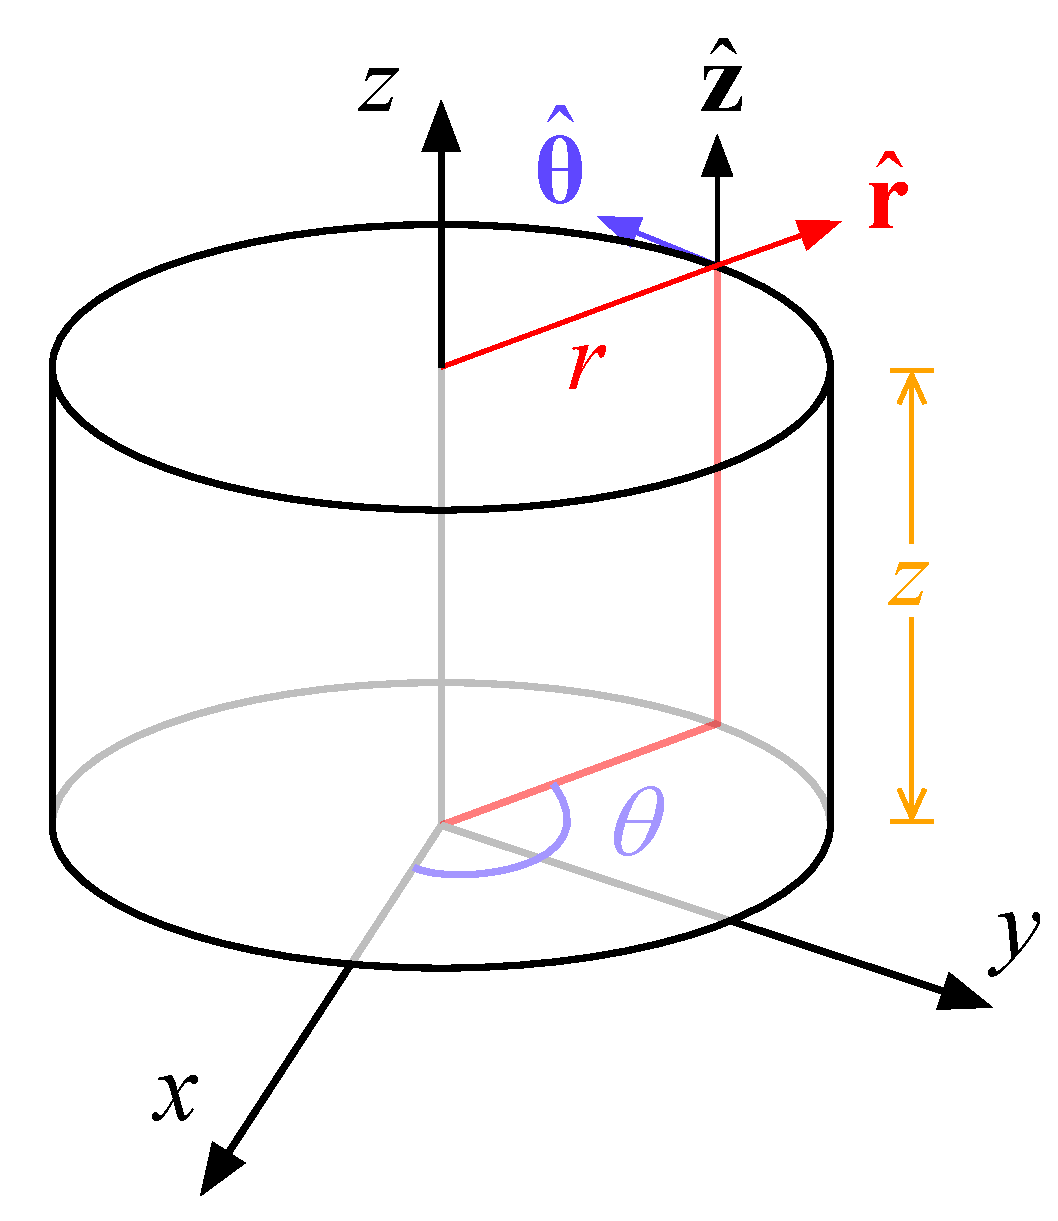
\includegraphics[width=4cm]{./figures/Cylin.pdf}
\caption{定义柱坐标系}\label{Cylin_fig1}
\end{figure}

\subsection{单位矢量}
柱坐标系中的单位矢量如\autoref{Cylin_fig1} 中的 $\uvec r,\uvec \theta ,\uvec z$ 所示.与直角坐标系不同的是,三个单位矢量与具体的坐标相关,不是常矢量.这在矢量求导时非常关键.

\subsection{与直角坐标系之间的变换}
根据三角函数相关定义以及勾股定理,显然有
\begin{equation}
\leftgroup{x &= r\cos \theta \\
y &= r\sin \theta \\
z &= z}
\qquad
\leftgroup{r &= \sqrt {x^2 + y^2} \\
\theta  &= \arctan 2\left( {x,y} \right)\\
z &= z}
\end{equation}
其中 $\arctan 2(x,y)$ 在第一四象限中就是我们熟知的 $\arctan (y/x)$, 但无法表示其他象限.为了解决这个问题,一些编程语言中加入了 $\arctan2$.这里将其定义为

\begin{equation}
\arctan 2(x,y) \equiv 
\leftgroup{
&\arctan (y/x) \quad &(x > 0)\\
&\pi /2 \quad &(x = 0, y > 0)\\
& - \pi /2 \quad &(x = 0, y < 0)\\
&\arctan (y/x) + \pi \quad &(x < 0,y \ge 0)\\
&\arctan (y/x) - \pi \quad &(x < 0,y < 0)
}
\end{equation}


















